\documentclass[a0paper,portrait]{baposter}

\usepackage{relsize}
\usepackage{url}
\usepackage{xspace}
\usepackage{subfig}
\usepackage{siunitx}
\usepackage{graphics}
\usepackage{enumitem}
\usepackage{amsmath}
\usepackage{color}

\graphicspath{./figures}

%%% Color Definitions %%%%%%%%%%%%%%%%%%%%%%%%%%%%%%%%%%%%%%%%%%%%%%%%%%%%%%%%%
\definecolor{bonngray}{cmyk}{0.0,0.00,0.15,0.55}   % HKS 95 (from style guide)
\definecolor{bonnyellow}{cmyk}{0.0,0.20,1.0,0.0}   % HKS 4 (from style guide)
\definecolor{bonnblue}{cmyk}{1.0,0.70,0.0,0.0}     % HKS 43 (from style guide)
\colorlet{bonnblue40}{bonnblue!50}
\colorlet{bonnblue20}{bonnblue!25}
\colorlet{bonngray50}{bonngray!50}
\colorlet{bonngray25}{bonngray!15}

%%% Utility functions %%%%%%%%%%%%%%%%%%%%%%%%%%%%%%%%%%%%%%%%%%%%%%%%%%%%%%%%%%
\newcommand{\compresslist}{
  \setlength{\itemsep}{1pt}
  \setlength{\parskip}{0pt}
  \setlength{\parsep}{0pt}
}
\newcommand{\TODO}[1]{\textcolor{red}{TODO: #1}}
\newcommand{\ie}{i.\,e.,\ }
\newcommand{\eg}{e.\,g.,\ }
\newcommand{\wrt}{w.r.t.\xspace}
\newcommand{\etal}{\xspace\textit{et~al.}\xspace}
\newcommand{\highlight}[1]{\textcolor{bonnblue}{#1}}
\newcommand{\HIGHLIGHT}[1]{\textcolor{bonnblue}{{\bf #1}}}
\newlength{\figureheight}
\newlength{\figurewidth}

%%%%%%%%%%%%%%%%%%%%%%%%%%%%%%%%%%%%%%%%%%%%%%%%%%%%%%%%%%%%%%%%%%%%%%%%%%%%%%% 
%%% Document Start %%%%%%%%%%%%%%%%%%%%%%%%%%%%%%%%%%%%%%%%%%%%%%%%%%%%%%%%%%%%
%%%%%%%%%%%%%%%%%%%%%%%%%%%%%%%%%%%%%%%%%%%%%%%%%%%%%%%%%%%%%%%%%%%%%%%%%%%%%%% 


\begin{document}
\typeout{Poster rendering started}

%%% Setting Background Image %%%%%%%%%%%%%%%%%%%%%%%%%%%%%%%%%%%%%%%%%%%%%%%%%%
\background{}

%%% General Poster Settings %%%%%%%%%%%%%%%%%%%%%%%%%%%%%%%%%%%%%%%%%%%%%%%%%%%
%%%%%% Eye Catcher, Title, Authors and University Images %%%%%%%%%%%%%%%%%%%%%%
\begin{poster}{
    grid=false,
    eyecatcher=true, 
    bgColorOne=white,
    bgColorTwo=white,
    borderColor=bonnblue,
    headerheight=0.07\textheight,
    headerColorOne=bonnblue,
    headerColorTwo=bonnblue,
    headerFontColor=white,
    boxColorOne=bonngray25,
    boxColorTwo=green,
    headershape=roundedright,
    headerfont=\Large\sf\bf,
    textborder=rectangle,
    background=user,
    headerborder=open,
    boxshade=plain
  }
  %%% Eye Cacther %%%%%%%%%%%%%%%%%%%%%%%%%%%%%%%%%%%%%%%%%%%%%%%%%%%%%%%%%%%%%%%
  {
    \includegraphics[height=4em]{pointcloudlibrary_vert_large_pos.png}
  }
  %%% Title %%%%%%%%%%%%%%%%%%%%%%%%%%%%%%%%%%%%%%%%%%%%%%%%%%%%%%%%%%%%%%%%%%%%%
  {\LARGE{\sf\bf
      Approximate Triangulation and Region Growing for Efficient Segmentation and Smoothing of Range Images
    }}
  %%% Authors %%%%%%%%%%%%%%%%%%%%%%%%%%%%%%%%%%%%%%%%%%%%%%%%%%%%%%%%%%%%%%%%%%%
  {
    \vspace{.5em}Dirk Holz, Autonomous Intelligent Systems, Computer Science VI
  }
  %%% Logo %%%%%%%%%%%%%%%%%%%%%%%%%%%%%%%%%%%%%%%%%%%%%%%%%%%%%%%%%%%%%%%%%%%%%%
  {
    \includegraphics[height=4em]{uni_logo.pdf}
  }
  

  \headerbox{Approach: simple but efficient processing pipeline}{name=approach,span=2,column=0,row=0}{
    \begin{center}
      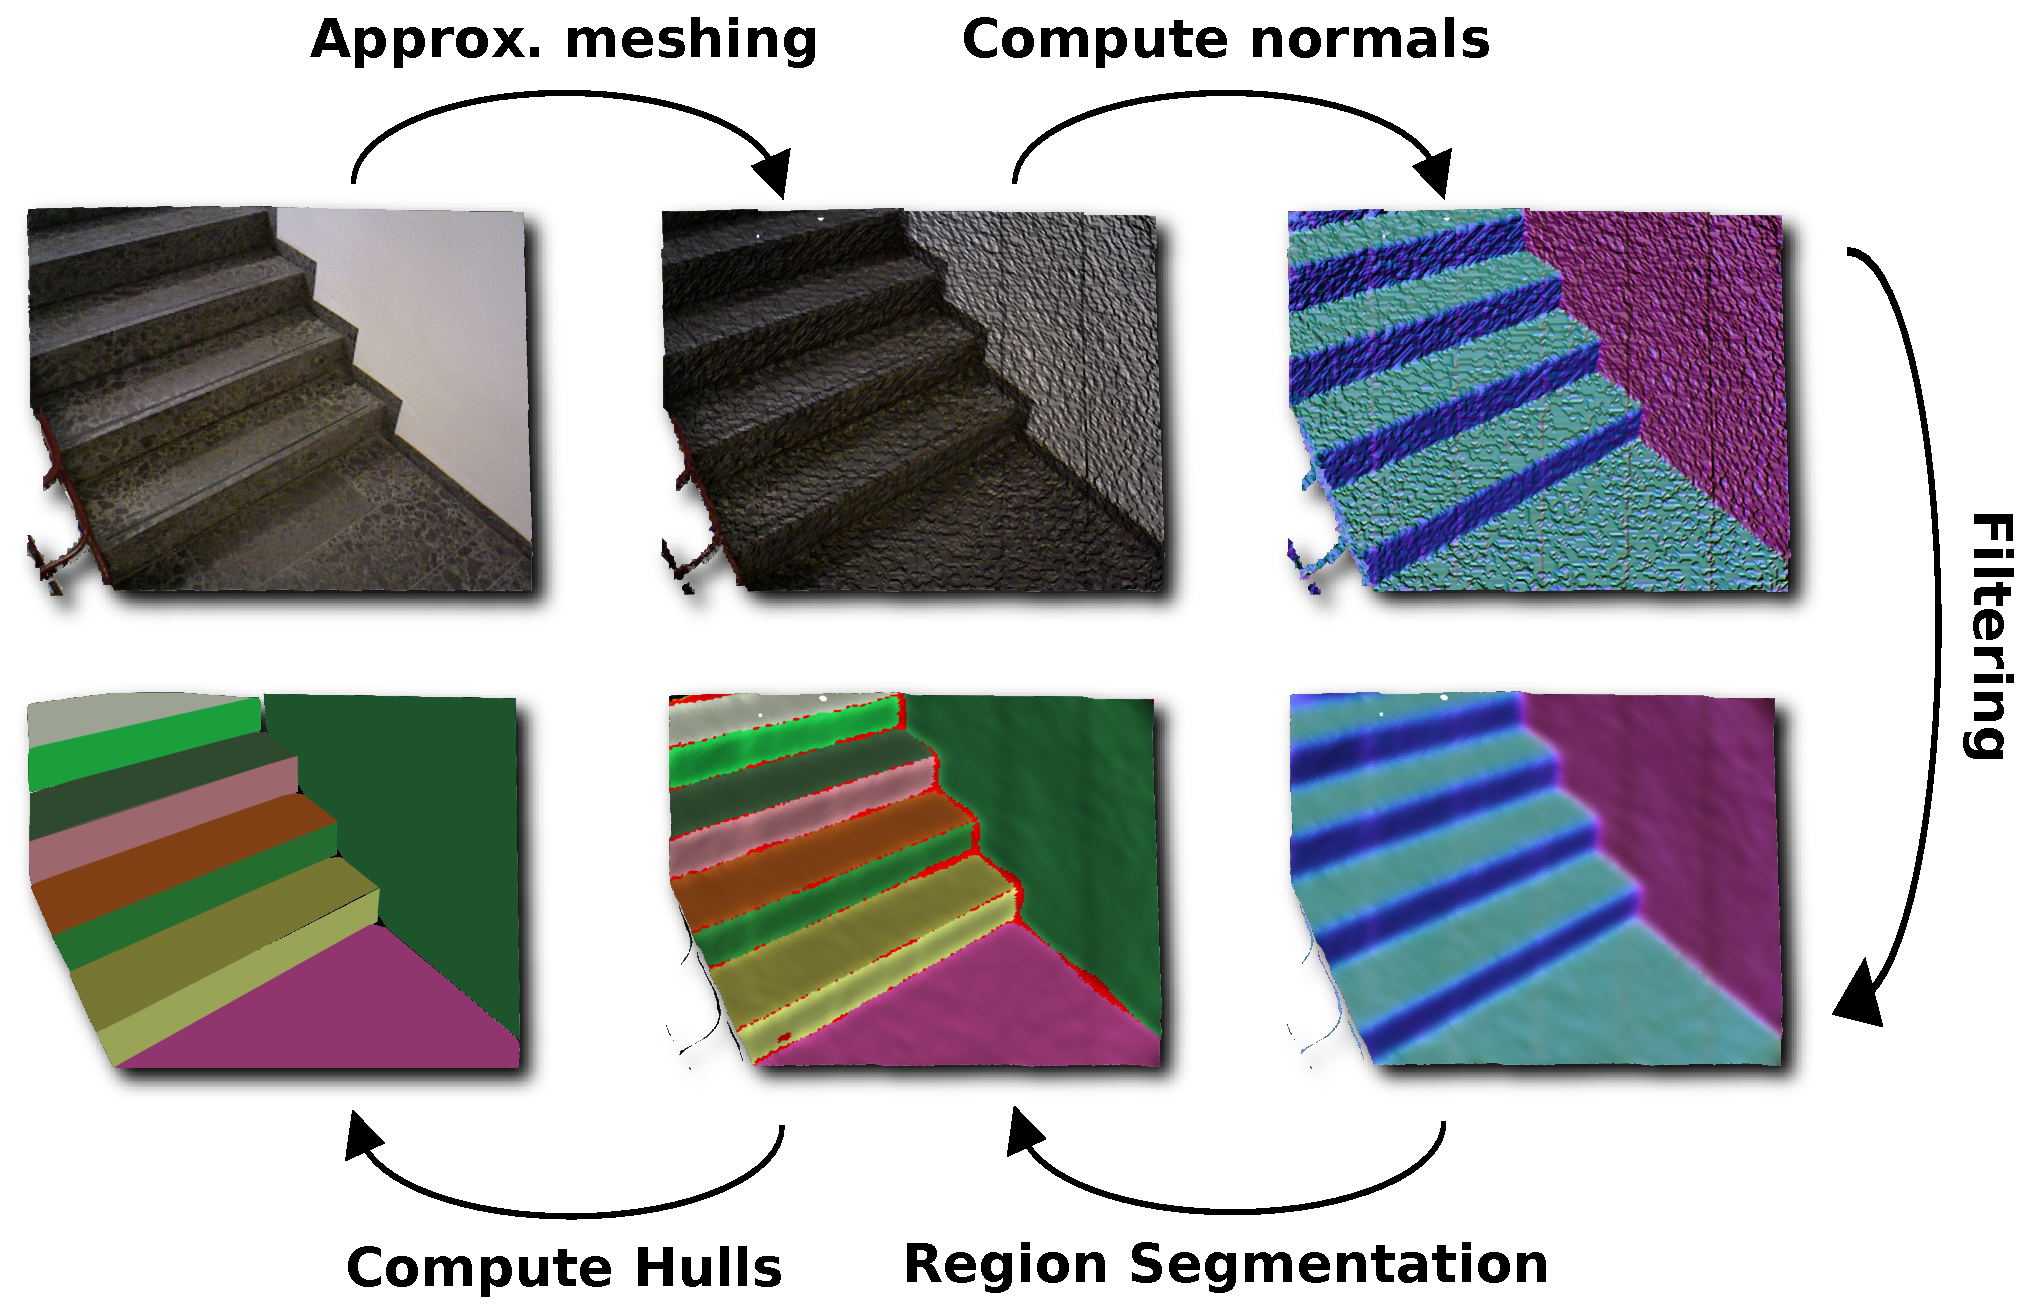
\includegraphics[width=0.921\linewidth]{approach_overview.pdf}
    \end{center}
    For an input organized point cloud or range image:
    \begin{enumerate}\compresslist
      \item we first deduce an \highlight{approximate triangle or quad mesh}, 
      \item efficiently highlight{compute local surface normals} and curvature directly on the mesh, 
      \item and \highlight{apply a multilateral filter} to smooth both the points and their normals.
      \item We \highlight{segment the smoothed mesh} into planar regions (and other geometric primitives).
    \end{enumerate}
  }

  \headerbox{Approximate triangulation}{name=meshing,span=1,column=2,row=0}{
    \begin{center}
      \begin{tabular}{cc}
        \includegraphics[clip,trim=1cm 1cm 1cm 1cm, width=.4\linewidth]{mesh_quad.pdf} & 
        \includegraphics[clip,trim=1cm 1cm 1cm 1cm, width=.4\linewidth]{tri_adaptive.pdf}\\[-.5em]
        Quad mesh & adaptive triangulation \\ 
        \includegraphics[clip,trim=1cm 1cm 1cm 1cm, width=.4\linewidth]{tri_right.pdf} & 
        \includegraphics[clip,trim=1cm 1cm 1cm 1cm, width=.4\linewidth]{tri_left.pdf} \\[-.5em]
        Only right cuts & left cuts
      \end{tabular}
      \begin{itemize}\compresslist
      \item The mesh is directly deduced from the image-like structure.
      \item Neighborhood relations are evaluated and cached in the mesh: for every \highlight{valid} point neighbors, we add an edge to the mesh.
        \begin{equation*}
          valid = \left( \left| \cos\theta_{i,j} \right| \le \cos\epsilon_\theta \right) \wedge \left( d_{i,j} \le \epsilon_d^2 \right), 
        \end{equation*}\vspace{-2em}
        \begin{eqnarray*}
          \text{with~~~~} \theta_{i,j} & = & \frac{\left( \mathbf{p}_i - \mathbf{f} \right) \cdot \left(\mathbf{p}_i - \mathbf{p_j}\right)}{\|\mathbf{p}_i - \mathbf{f}\|\ \|\mathbf{p}_i - \mathbf{p_j}\|},\\
          \text{and~~~~~~~} d & = & \|\mathbf{p}_i - \mathbf{p_j}\|^2, 
        \end{eqnarray*}
        with normal deviation tolerance $\epsilon_\theta$ and distance tolerance $\epsilon_d$.
      \end{itemize}
    \end{center}
  }


  \headerbox{Surface Normals}{boxColorOne=white,boxColorOne=white,name=normals,column=0,below=approach}{
    We compute the local surface normal $\mathbf{n}_i$ for point $\mathbf{p}_i$ as the weighted average of the plane normals of the $N_T$ faces surrounding $\mathbf{p}_i$.
    \begin{equation}
      \mathbf{n}_i = \frac{\sum_{j=0}^{N_T}(\mathbf{p}_{j,a}-\mathbf{p}_{j,b}) \times (\mathbf{p}_{j,a}-\mathbf{p}_{j,c})}{\|\sum_{j=0}^{N_T}(\mathbf{p}_{j,a}-\mathbf{p}_{j,b}) \times (\mathbf{p}_{j,a}-\mathbf{p}_{j,c})\|}, 
    \end{equation}
    where $\mathbf{p}_{j,a}$, $\mathbf{p}_{j,b}$ and $\mathbf{p}_{j,c}$ form triangle $j$.
  }


  \headerbox{Multilateral Filtering}{boxColorOne=white,name=filtering,column=0,below=normals}{
    for smoothing both the points and their normals while preserving edges in the sensed geometric structures.
    {\smaller
      \begin{equation*}
        \mathbf{p}_i\!=\!\sum_{j \in N_i} w_{ij}\mathbf{p_i}\!/\!\sum_{j \in N_i} w_{ij}, \ \text{and~}
        \mathbf{n}_i\!=\!\sum_{j \in N_i} w_{ij}\mathbf{n_i}\!/\!\sum_{j \in N_i} w_{ij}, \quad
      \end{equation*}
    }
    \begin{equation*}
      w_{ij} = \underbrace{e^{\alpha\|\mathbf{p}_i - \mathbf{p_j}\|}}_{\text{distance term}}\; 
      \underbrace{e^{\beta\|\mathbf{n}_i - \mathbf{n}_j\|_1}}_{\text{normal term}}\;\: 
      \underbrace{e^{\gamma(I_i - I_j)/c_I}}_{\text{intensity term}}.
    \end{equation*}
    \begin{center}
      \includegraphics[width=.75\linewidth]{filtering_details.pdf}
    \end{center}
  }


  \headerbox{Region Growing}{boxColorOne=white,name=segmentation,column=0,below=filtering}{
    to segment \textcolor{cyan!90!black}{cylinders}, \textcolor{yellow!90!black}{planes}, and \textcolor{pink!90!black}{spheres}:
    \begin{center}
      \includegraphics[clip,trim=0.5cm 0cm 2cm 0cm,width=.48\linewidth]{prim_det_1.png}
      \includegraphics[clip,trim=2cm 3cm 5cm 1.5cm,width=.48\linewidth]{prim_det_2.png}
    \end{center}
  }



  \headerbox{Experiments and Results \cite{holz_2012_ias,holz_ras_si_ias}}{boxColorOne=white,name=results,span=2,column=1,below=approach}{

    \begin{center}
      \begin{tabular}{ccccc}
        \multicolumn{4}{l}{{\bf Plane segmentation in range images:} (SegComp data sets)}\\
        \includegraphics[height=.17\linewidth]{perceptron_test_5.png} & 
        \includegraphics[height=.17\linewidth]{perceptron_test_6.png} & 
        \includegraphics[height=.17\linewidth]{perceptron_test_7.png} & 
        \includegraphics[height=.17\linewidth]{perceptron_test_8.png} & 
        \includegraphics[height=.17\linewidth]{perceptron_test_9.png} \\[-.3em]
        10/14 & 18/24 & 10/13 & 12/13 & 22/22\\[.5em]
        \includegraphics[height=.17\linewidth]{abw_test_25.png} & 
        \includegraphics[height=.17\linewidth]{abw_test_26.png} & 
        \includegraphics[height=.17\linewidth]{abw_test_27.png} & 
        \includegraphics[height=.17\linewidth]{abw_test_28.png} & 
        \includegraphics[height=.17\linewidth]{abw_test_29.png} \\[-.3em]
        10/11 & 9/10 & 9/9 & 8/8 & 8/10\\
      \end{tabular}
    % \end{center}

    % \begin{center}
      \begin{tabular}{cccc}
        \multicolumn{4}{l}{{\bf Cylinder segmentation in Kinect data:}}\\
        \includegraphics[height=.16\linewidth]{kinect_cylinders_29_seg.jpg} & 
        \includegraphics[height=.16\linewidth]{kinect_cylinders_14_seg.jpg} & 
        \includegraphics[height=.16\linewidth]{kinect_cylinders_12_seg.jpg} & 
        \includegraphics[height=.16\linewidth]{kinect_cylinders_19_seg.jpg} \\[-.3em]
        2/2 & 3/3 & 4/4 & 4/6\\
      \end{tabular}

      \begin{tabular}{ll}
        {\bf Runtime evaluation} & {\bf Noise model} (for $\epsilon_d$)\\
        \includegraphics[height=.15\linewidth]{results_runtime.png} \hspace{3cm} & 
        \includegraphics[clip,trim=0cm 0cm 2cm 0cm,  height=.17\linewidth]{kinect_noise.jpg}
        \includegraphics[clip,trim=0cm 0cm 12cm 0cm, height=.17\linewidth]{kinect_noise_detail.jpg}
      \end{tabular}
      
    \end{center}




    \textbf{Results:} \HIGHLIGHT{State-of-the-art performance while being significantly faster}.
  }


  \headerbox{References}{name=references,span=2,column=1,below=results}{
    \smaller
    \vspace{-0.4em}
    \bibliographystyle{./style/IEEEbib}
    \begingroup
    \renewcommand{\section}[2]{}%
    \bibliography{references}
    \endgroup
  }


\end{poster}
\end{document}
